\documentclass[a4paper, 12pt]{article}

% -- Language --
\usepackage[spanish]{babel}
\usepackage[utf8]{inputenc}

% ----- Fonts -----
% -- Fuente --
\usepackage{fontspec}
\setmonofont{JetBrainsMono Nerd Font}  

% -- Color --
\usepackage{xcolor}
%\definecolor{azul}{RGB}{00,33,99}
\definecolor{azul}{RGB}{35,72,180}

% -- Page Margin --
\usepackage[margin=1in]{geometry}

% -- Espaciados --
\newcommand{\Pspace}{0.5cm}
\newcommand{\Aspace}{0.2cm}

% -- Imagenes --
\usepackage{graphicx}
\usepackage{float}

% -- Matemáticas --
\usepackage{amsmath, amssymb}

% -- Gráficas --
\usepackage{pgfplots}
\pgfplotsset{compat=1.18}

% -- Código --
\usepackage{listings}
\lstset{
    language=C++,                   % Lenguaje del código
    basicstyle=\ttfamily\small,     % Fuente del código
    keywordstyle=\color{blue},      % Color de palabras clave
    commentstyle=\color{gray},      % Color de comentarios
    stringstyle=\color{red},        % Color de cadenas
    numbers=left,                   % Números de línea a la izquierda
    numberstyle=\tiny\color{gray},
    breaklines=true,                % Permitir saltos de línea
    frame=single                    % Marco alrededor del código
}


\title
{
    Diseño de Sistemas Digitales 2025-2 \\
    Problemas Unidad 1
}

    \begin{document}

    \maketitle

    \begin{center}
        \begin{tabular}{r|l}
            \textbf{Expediente} & \textbf{Nombre} \\ \hline
            219208106 & Bórquez Guerrero Angel Fernando \\
        \end{tabular}
    \end{center}

    \rule{\linewidth}{0.3mm}



    \vspace{0.3cm}
    \begin{enumerate}
        % - Problema 1
        \item Escriba la expresión booleana para la salida $X$ en la figura. Determine el valor de $X$ para todas las posibles condiciones de entrada y liste los valores en una tabla de verdad. \par
        \begin{figure}[!ht]
            \centering
            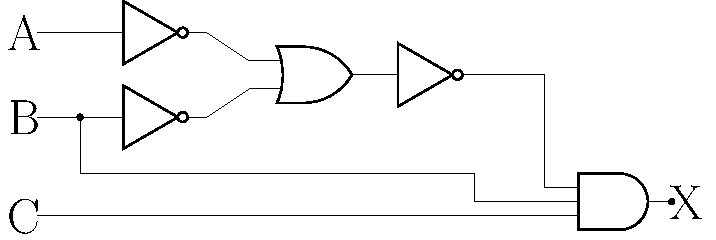
\includegraphics[width=0.5\textwidth]{Circuitos/Figuras/Figura_1.pdf}
        \end{figure}
            % Respuestas:
            \vspace{\Aspace} \par
            {   \color{azul} Expresión: $\overline{(\bar{A}+\bar{B})}BC$ \par \vspace{0.5cm}
                \begin{tabular}{c|c|c|c}
                    \textbf{A}  &   \textbf{B}  &   \textbf{C}  &   $\overline{(\bar{A}+\bar{B})}BC$    \\ \hline
                    1           &   1           &   1           &   1                                   \\
                    1           &   1           &   0           &   0                                   \\
                    1           &   0           &   1           &   0                                   \\
                    1           &   0           &   0           &   0                                   \\
                    0           &   1           &   1           &   0                                   \\
                    0           &   1           &   0           &   0                                   \\
                    0           &   0           &   1           &   0                                   \\
                    0           &   0           &   0           &   0                                   \\
                \end{tabular}
            }


        \newpage
        % - Problema 2
        \item Repita el proceso del problema anterior para el circuito de la siguiente figura. \par
        \begin{figure}[!ht]
            \centering
            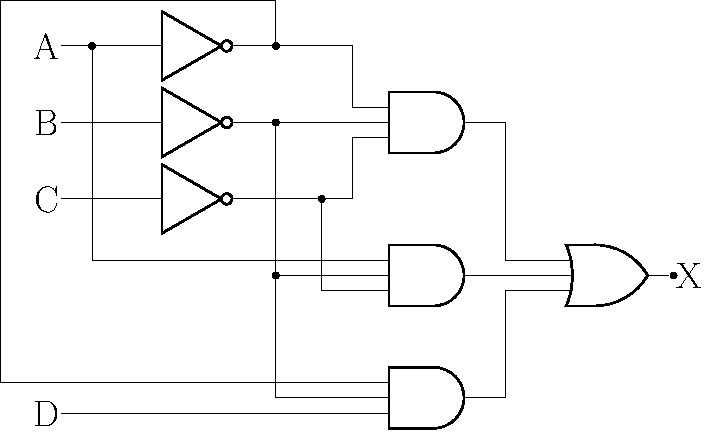
\includegraphics[width=0.5\textwidth]{Circuitos/Figuras/Figura_2.pdf}
        \end{figure}
            % Respuesta:
            \vspace{\Aspace} \par
            { \color{azul} Expresión: $(\bar{A} \bar{B} \bar{C}) + (A \bar{B} \bar{C}) + (\bar{A} \bar{B} D)$ \par \vspace{0.5cm}
                \begin{tabular}{c|c|c|c|c}
                    \textbf{A}  &   \textbf{B}  &   \textbf{C}  &   \textbf{D}  &   $(\bar{A} \bar{B} \bar{C}) + (A \bar{B} \bar{C}) + (\bar{A} \bar{B} D)$     \\ \hline
                    1           &   1           &   1           &   1           &   0                                                                           \\
                    1           &   1           &   1           &   0           &   0                                                                           \\
                    1           &   1           &   0           &   1           &   0                                                                           \\
                    1           &   1           &   0           &   0           &   0                                                                           \\
                    1           &   0           &   1           &   1           &   0                                                                           \\
                    1           &   0           &   1           &   0           &   0                                                                           \\
                    1           &   0           &   0           &   1           &   1                                                                           \\
                    1           &   0           &   0           &   0           &   1                                                                           \\
                    0           &   1           &   1           &   1           &   0                                                                           \\
                    0           &   1           &   1           &   0           &   0                                                                           \\
                    0           &   1           &   0           &   1           &   0                                                                           \\
                    0           &   1           &   0           &   0           &   0                                                                           \\
                    0           &   0           &   1           &   1           &   1                                                                           \\
                    0           &   0           &   1           &   0           &   0                                                                           \\
                    0           &   0           &   0           &   1           &   1                                                                           \\
                    0           &   0           &   0           &   0           &   1                                                                           \\
                \end{tabular} 
            }



        % - Problema 3
        \item Para cada una de las siguientes expresiones, construya el circuito lógico correpondiente utilizando compuertas AND y OR e INVERSIONES.
             % Respuestas:
            \vspace{\Aspace} \par
            a) $y = (\bar{M} + \bar{N} + \overline{PQ})$
            \\ { \color{azul} 
                \begin{figure}[!ht]
                    \centering
                    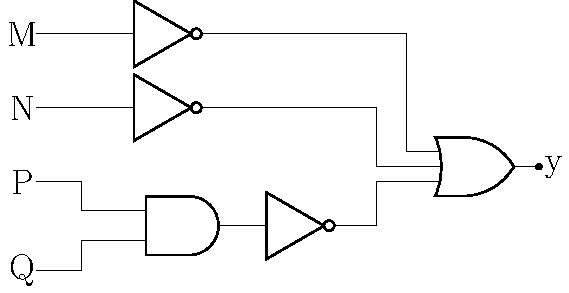
\includegraphics[width=0.6\textwidth]{Circuitos/Respuestas/Respuesta_3a.pdf}
                \end{figure}
            }

            \vspace{\Aspace} \par
            b) $x = \overline{W + P\bar{Q}}$
            \\ { \color{azul} 
                \begin{figure}[!ht]
                    \centering
                    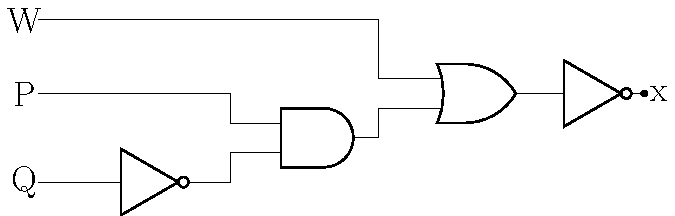
\includegraphics[width=0.6\textwidth]{Circuitos/Respuestas/Respuesta_3b.pdf}
                \end{figure}
            }

            \vspace{\Aspace} \par
            c) $z = MN(P + \bar{N})$
            \\ { \color{azul} 
                \begin{figure}[!ht]
                    \centering
                    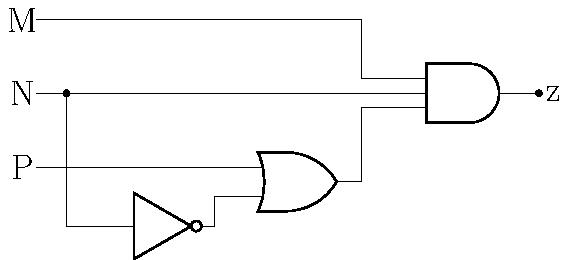
\includegraphics[width=0.6\textwidth]{Circuitos/Respuestas/Respuesta_3c.pdf}
                \end{figure}
            }

            \vspace{\Aspace} \par
            d) $x = (A + B)(\bar{A} + \bar{B})$
            \\ { \color{azul} 
                \begin{figure}[!ht]
                    \centering
                    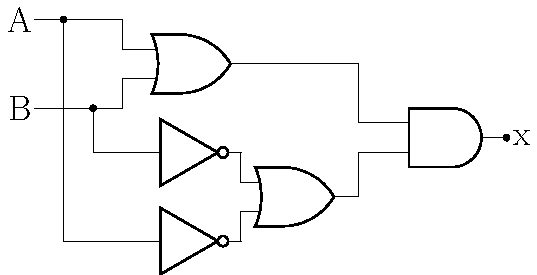
\includegraphics[width=0.6\textwidth]{Circuitos/Respuestas/Respuesta_3d.pdf}
                \end{figure}
            }



        \newpage
        % - Problema 4
        \item Escriba la expresión para la salida del circuito de la figura y utilícela para determinar la tabla de verdad completa.
        \begin{figure}[!ht]
            \centering
            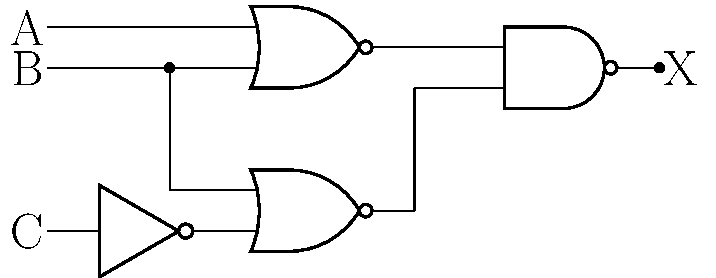
\includegraphics[width=0.5\textwidth]{Circuitos/Figuras/Figura_4.pdf}
        \end{figure}
            % Respuesta:
            \vspace{\Aspace} \par
            {   \color{azul} Expresión: $\overline{\overline{(A + B)} \cdot \overline{(B + \bar{C})}}$ \par \vspace{0.5cm}
                \begin{tabular}{c|c|c|c}
                    \textbf{A}  &   \textbf{B}  &   \textbf{C}  &   $\overline{\overline{(A + B)} \cdot \overline{(B + \bar{C})}}$     \\ \hline
                    1           &   1           &   1           &   1                                                           \\
                    1           &   1           &   0           &   1                                                           \\
                    1           &   0           &   1           &   1                                                           \\
                    1           &   0           &   0           &   1                                                           \\
                    0           &   1           &   1           &   1                                                           \\
                    0           &   1           &   0           &   1                                                           \\
                    0           &   0           &   1           &   0                                                           \\
                    0           &   0           &   0           &   1                                                           \\
                \end{tabular}
            }
        


        % - Problema 5
        \item Completa cada una de las expresiones.
            % Respuestas:
            \vspace{\Aspace} \par
            a) $A + 1 = $
            { \color{azul} $1$ }

            \vspace{\Aspace} \par
            b) $A \cdot A = $
            { \color{azul} $A$ }

            \vspace{\Aspace} \par
            c) $B \cdot \bar{B} = $
            { \color{azul} $0$ }

            \vspace{\Aspace} \par
            d) $C + \bar{C} = $
            { \color{azul} $1$ }

            \vspace{\Aspace} \par
            e) $x \cdot 0 = $
            { \color{azul} $0$ }

            \vspace{\Aspace} \par
            f) $D \cdot 1 = $
            { \color{azul} $D$ }

            \vspace{\Aspace} \par
            g) $D + 0 = $
            { \color{azul} $D$ }

            \vspace{\Aspace} \par
            h) $C + C = $
            { \color{azul} $C$ }

            \vspace{\Aspace} \par
            i) $G + GF = $
            { \color{azul} $G$ }

            \vspace{\Aspace} \par
            j) $y + wy = $
            { \color{azul} $y$ }


        \newpage
        % - Problema 6
        \item Simplifique la siguiente expresión usando los teoremas (3), (4) y (13b).
        \\ (3) $x \cdot x = x$
        \\ (4) $x \cdot \bar{x} = 0$
        \\ (13b) $(w + x)(y + z) = wy + wz + xy + xz$
        \[ x = (M + N)(\bar{M} + P)(\bar{N} + \bar{P})\]
            % Respuesta:
            \par
            { \color{azul} 
                        $(M\bar{M} + MP + \bar{M}N + NP)(\bar{N} + \bar{P})$
                \par    $(MP + \bar{M}N + NP)(\bar{N} + \bar{P})$
                \par    $M\bar{N}P + MP\bar{P} + \bar{M}N\bar{N} + \bar{M}N\bar{P} + N\bar{N}P + NP\bar{P}$
                \par    $M\bar{N}P + \bar{M}N\bar{P}$
            }


        
        % - Problema 7
        \item Simplifique la siguiente expresión utilizando los teoremas (13a), (8) y (6):
        \[ z = \bar{A}B\bar{C} + AB\bar{C} + B\bar{C}D \]
            % Respuesta:
            \par
            { \color{azul} 
                        $B\bar{C}(\bar{A} + A + D)$
                \par    $B\bar{C}(1 + D)$
                \par    $B\bar{C}(D)$
                \par    $B\bar{C}$
            }



        % - Problema 8
        \item Simplifique cada una de las siguientes expresiones usando lso teoremas de DeMorgan.
            % Respuestas:
            \vspace{\Aspace} \par
            a) $\overline{\bar{A} + \bar{B}C}$
            \\ { \color{azul} $AB + \bar{C}$ }

            \vspace{\Aspace} \par
            b) $\overline{A + \bar{B}}$
            \\ { \color{azul} $\bar{A}B$ }

            \vspace{\Aspace} \par
            c) $\overline{\bar{A} + \bar{C} + \bar{D}}$
            \\ { \color{azul} $ACD$ }

            \vspace{\Aspace} \par
            d) $\overline{(M + \bar{N})(\bar{M} + N)}$
            \\ { \color{azul} $\bar{M}N + M\bar{N}$ }

            \vspace{\Aspace} \par
            e) $\overline{\overline{AB}CD}$
            \\ { \color{azul} $AB + \bar{C} + \bar{D}$ }


        
        \newpage
        % - Problema 9
        \item Un jet emplea un sistema para monitorear los valores de revoluciones por minuto (rpm), presión y temperatura de sus motores mediante el uso de motores que operan de la siguiente manera:
        \begin{itemize}
            \item Salida del sensor de $RPM = 0$ solo cuando la velocidad < 4800 rpm.
            \item Salida del sensor $P = 0$ solo cuando la presión < 220 psi.
            \item Salida del sensor $T = 0$ solo cuando la temperatura 200$\textdegree F$.
        \end{itemize}
        La figura muestra el circuito lógico que controla una luz de advertencia en cabina para ciertas combinaciones de condiciones del motor. Suponga que el nivel ALTO en la salida $W$ activa la luz de advertencia.
        \begin{figure}[!ht]
            \centering
            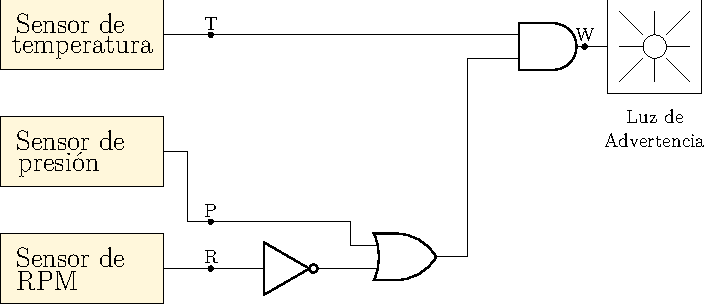
\includegraphics[width=0.7\textwidth]{Circuitos/Figuras/Figura_9.pdf}
        \end{figure}
            % Respuestas:
            \vspace{\Aspace} \par
            a) Determine qué condiciones del motor darán una advertencia al piloto.
            \\ { \color{azul} 
                Expresión de salida: $T(P + \bar{R})$
                \par Condiciones necesarias:
                \par 1. $T \geq 200\textdegree F$, $P \geq 220$psi y $R < 4800$rpm.
                \par 2. $T \geq 200\textdegree F$, $P \geq 220$psi y $R \geq 4800$rpm.
                \par 3. $T \geq 200\textdegree F$, $P < 220$psi y $R < 4800$rpm.
            }

            \vspace{\Aspace} \par
            b) Cambie este circuito por uno que utilice sólo compuertas NAND.
            \\ { \color{azul}
                \begin{figure}[!ht]
                    \centering
                    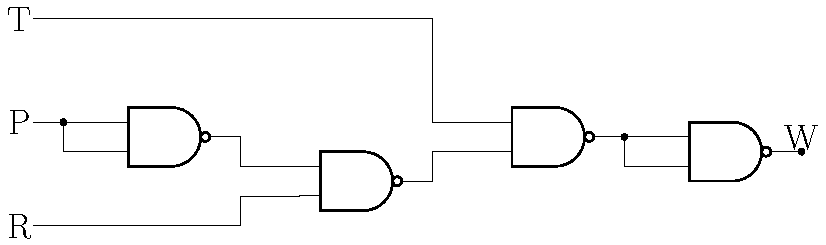
\includegraphics[width=0.7\textwidth]{Circuitos/Respuestas/Respuesta_9b.pdf}
                \end{figure}
                \par Expresión: $\overline{\left[ \overline{\left(T  \overline{\left(\overline{(P P)} R\right)}\right)} \cdot \overline{\left(T  \overline{\left(\overline{(P P)} R\right)}\right)} \right]} \equiv T(P + \bar{R})$
            }



        \newpage
        % - Problema 10
        \item Determina las condiciones de entrada necesarias para hacer que la salida en la figura cambie a su estado activo.
        \begin{figure}[!ht]
            \centering
            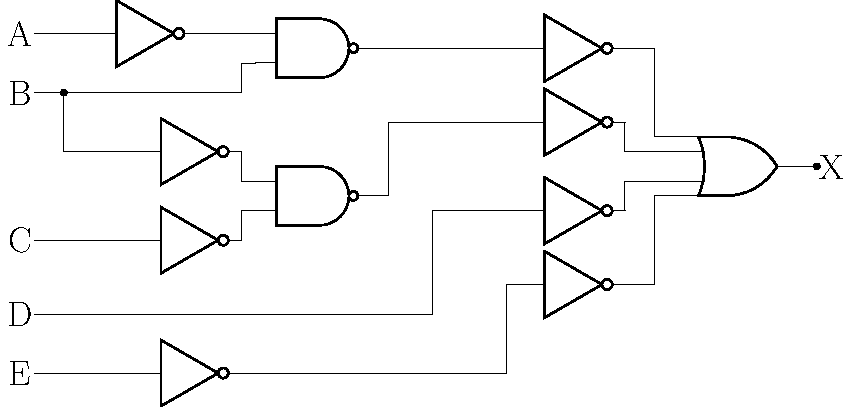
\includegraphics[width=0.7\textwidth]{Circuitos/Figuras/Figura_10.pdf}
        \end{figure}
            % Respuesta:
            \vspace{\Aspace} \par
            { \color{azul} 
                Expresión: $\overline{\overline{(\overline{A}B)}} + \overline{\overline{(\bar{B}\bar{C})}} + \overline{D} + \overline{\overline{E}} \equiv (\overline{A}B) + (\bar{B}\bar{C}) + \overline{D} + E$
                \par Condiciones necesarias:
                \par 1. $A = 0$ y $B = 1$
                \par 2. $B = 0$ y $C = 0$
                \par 3. $D = 0$
                \par 4. $E = 1$
            }



        % - Problema 11
        \item La figura muestra una aplicación de compuertas lógicas que simula un interruptor de dos vías, como los que utilizamos en nuestros hogares para encender o apagar una luz desde dos interruptores distintos. Aquí la luz es un LED que estará ENCENDIDO (en conducción) cuando la salida de la compuerta NOR esté en BAJO. Observe que esta salida está etiquetada como LUZ para indicar que es activa en BAJO. Determine las condiciones de entrada necesarias para encender el LED. Después verifique que el circuito opere como un interruptor de dos vías, utilizando los interruptores A y B.
        \begin{figure}[!ht]
            \centering
            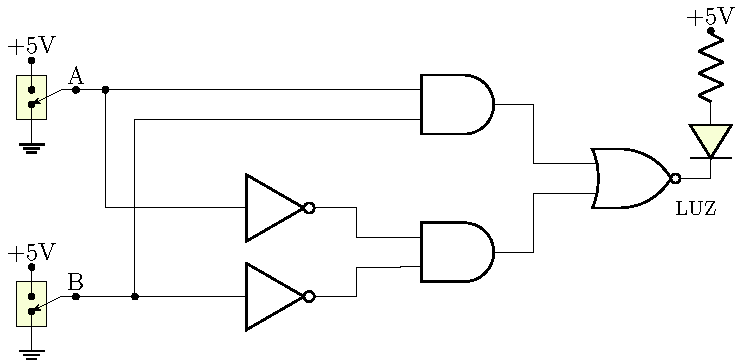
\includegraphics[width=0.7\textwidth]{Circuitos/Figuras/Figura_11.pdf}
        \end{figure}
            % Respuestas:
            { \color{azul} 
                \par Expresión: $\overline{AB + \bar{A}\bar{B}}$
                \par Condiciones necesarias:
                \par 1. $A = 1$ y $B = 0$
                \par 2. $A = 0$ y $B = 1$
            }



    \end{enumerate}
\end{document}
